% !TeX root = scaffold-50.tex
\renewcommand{\imagepath}{../50-unsupervised/img}
\newcommand{\ntopics}{n_\text{topics}}

\chapter{Unsupervised Analysis: Topic Modelling}
In this chapter, the topics of the celebrity newspaper articles are examined using the topic modelling technique. After showing that using \gls{lda} alone does not yield robust and reliable results, semantic-similarity clustering is shown to improve the quality of the topic extraction.  Finally, the significance of differences in the topic distributions of low-\gls{ses} and high-\gls{ses} newspaper articles are discussed.

The main focus is to find the prevailing topics in the celebrity newspaper articles and to examine any differences in the distribution of these topics between the low-\gls{ses} and high-\gls{ses} groups.\todo{Motivate more again}

\section{Shortcomings of \gls{lda} Topic Modelling}
In a first attempt, \gls{lda} model instances (see chapter~\ref{ch:lda}) were trained for a varying number of topics $\ntopics$. The corpus of all relevant newspaper articles comprised the 50-article balanced data set ensuring that role models with many articles could not induce a topic bias in the models. The texts were fed to the models in the \textit{noun and verb} stage in order to focus on the meaning-bearing elements of the texts.

Each of these model instances yielded a set of $\ntopics$ topics. Each topic $t$ is defined by a list $T_{\ntopics, t}$ of characterizing topic words. Each model assigned to every newspaper article $i$ estimated probabilities $p_{i, t}$ that article $i$ would belong to the topic $t$. Each newspaper article $i$ was assigned a topic $t_i$ by selecting the topic with the maximum probability:
\begin{align}
    t_i = \arg \max_{t'} p_{i, t'}
\end{align}

Figure~\ref{fig:topic_modelling_schema} illustrates the modelling and assigment process.
\begin{figure}
    \centering
    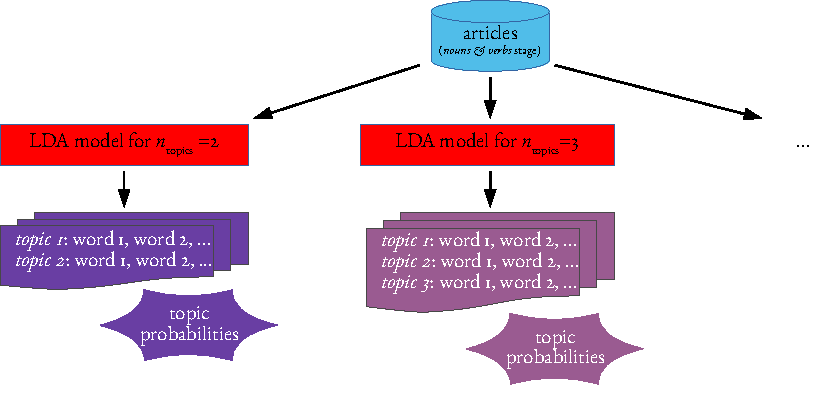
\includegraphics[]{\imagepath/topic_modelling_schema.pdf}
    \caption{Schematic of the topic modelling setup with \gls{lda}: Many models for different numbers $\ntopics$ of topics are trained, each of them yields a list of topics that are characterized by topic words, as well as topic probabilities for each article.}\label{fig:topic_modelling_schema}
\end{figure}

The \gls{lda} algorithm depends on a set of hyperparameters, most of which are related to its underlying optimization process.  Sensible values for these were found by trial and error. The one hyperparameter that is crucial for the interpretation of this analysis is $\ntopics$. It determines the granularity of the topics the model provides for the comparison of the low- and high-\gls{ses} groups. The trade-off between a low and a high number of topics is expected to be a well-graspable set of topics with considerable overlaps and therefore poor specificity for low $\ntopics$, in contrast to highly delimited niche-topics suffering from a lack of generality for high $\ntopics$. For choosing an appropriate $\ntopics$ in this work, it was required that the topics assigned to articles be consistent for small variations of $\ntopics$, since only then it can be assumed that the assignment of the articles to the low- and high-\gls{ses} groups will not just be a random effect. The search for an optimal number of topics included introducing of so-called \textit{hypertopics} to make model output topics comparable as well as assessing ranges for $\ntopics$ with respect to hypertopic accuracy and consistency of the \gls{ses} assignment.

\paragraph{Assigning Hypertopics}
As the model output topics are only defined by a list of characterizing words, the individual topics can overlap in term of their meaning (e.g. different kinds of sport), and the topics obtained for different $\ntopics$ cannot be compared without human intuition. In order to still be able to compare the model outputs for different $\ntopics$, each topic was manually assigned one of the four \textit{hypertopics} movie, music, sport, and life (with life being intended as a miscellaneous category for all topics not covered by the other three hypertopics). These four hypertopics were heuristically selected while examining the model output topics. Each article $i$ with topic $t$ was by that means also assigned a hypertopic $h$:
\begin{align}
    h_i = h(t_i)
\end{align}
Table~\ref{tab:hypertopics} shows examples of the model output topics and their manually assigned hypertopics and shows the generality vs specificity trade-off in terms of the chosen $\ntopics$.

\begin{table}
    \centering
    \begin{tabular}{clc}
        \toprule
        $\ntopics$ & topic words for exemplary topics (model output) & hypertopic \\
        \toprule 
        \multirow{3}{*}{5} & love video fan people thing song feel music share life & \textit{life}\\
        & game player team season goal win league sport club score & \textit{sport}\\
        & film llc st ave dr series movie season actor michael & \textit{movie}\\
        \midrule
        \multirow{3}{*}{50} & music artist business sony continue record label company team partner & \textit{music} \\
        & inc property water art road town science management development site & \textit{life} \\
        & fc week injury season run football quarter marcel yard dortmund & \textit{sport} \\
        \bottomrule
    \end{tabular}
    \caption{Example of model output topics and their respective hypertopics. Comparing the \textit{sport} hypertopic examples for $\ntopics = 5$ and $\ntopics = 50$ shows how a larger amount of model topics makes the topics more specific, here by referencing a particular sport and a particular sports club.}\label{tab:hypertopics}
\end{table}

With every article associated to a hypertopic, it is possible to compare the distribution of articles and \gls{ses} groups across hypertopics for different $\ntopics$ as well as verifying topic assignments with the human-annotated data.

\paragraph{Accuracy and Consistency}
In the next step, the accuracy of the topic models was assessed with the human-annotated data and the consistency of the predictions for different $\ntopics$.

The accuracy of the hypertopic assignment was calculated as the ratio of articles with correct hypertopic assignment by the model and all articles that were human-annotated:
\begin{align}
    acc = \frac{
        \left|
            \left\{i\middle|h_{i}^\text{predicted} = h_{i}^\text{true}\right\}
        \right|
    }{
        \left|
            \{{i|i \text{ was human-annotated}}\}
        \right|
    }
\end{align}

Figure~\ref{fig:accuracy_by_ntopics} reveals that the accuracy is not steady across different $\ntopics$ and comparably low.

\begin{figure}
    \centering
    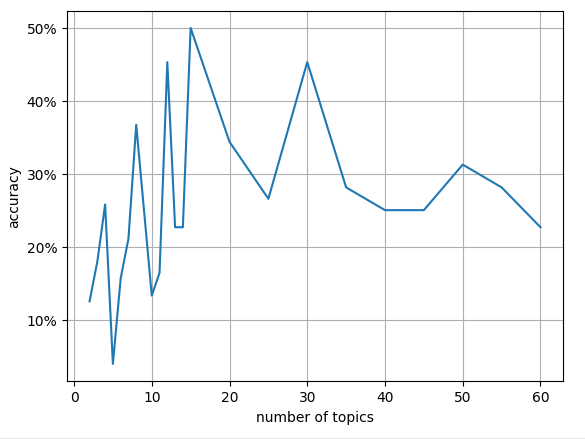
\includegraphics[scale=0.5]{\imagepath/acc_by_n_topic_modelling.png}
    \caption{Accuracy of the model-assigned hypertopics compared to human-annotated data as a function of the number of topics: The accuracy is comparably low and not consistent across the different numbers of topics.\todo[inline]{replace}}\label{fig:accuracy_by_ntopics}
\end{figure}

Additionally, the share of low-\gls{ses} articles for each assigned hypertopic was used as a measure for topic assignment consistency across $\ntopics$. This share is plotted in figure~\ref{fig:lowshare_per_ntopics}. The fact that there is no range of $\ntopics$ where this share is consistent for small variations of $\ntopics$ suggests that the assignment of articles to the hypertopics is to a considerable extent random and that the model is incapable of making a reliable prediction of an article's topic.\todo{Explain more why you took exactly this share and not anything else.}

\begin{figure}
    \centering
    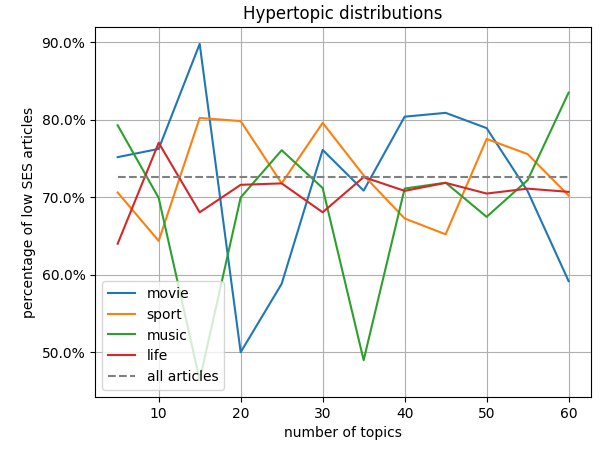
\includegraphics[scale=0.5]{img/low_ses_by_n_topic_modelling.png}
    \caption{Share of low-\gls{ses} articles in each hypertopic across different numbers of topics: The share is not consistent over a range from \SI{5}{} to \SI{50}{} topics, indicating that the assigment of articles to topics is not very reliable.\todo[inline]{replace}}\label{fig:lowshare_per_ntopics}
\end{figure}

The author guesses that one of the reasons for these inconsistent variations in topic assignment is the newspaper articles operate on a very limited set of topics, roughly covered by the for hypertopics, which do expose considerable overlaps (e.g. movie-related articles having similarity to life stories, film music-related articles talking about movies). This could render the topic models incapable of capturing distinct groups of articles, rather than assigning topics seemingly randomly.

As a potential fix, training topic models on the low-\gls{ses} and high-\gls{ses} corpora separately was tried, but led to similar inconsistencies. Instead, the topic modelling approach was enhanced by the use of a pretained transformer model as described in the next section.

\section{Improvement with Semantic Embeddings}

\section{Discussion}